\documentclass[a4paper,11pt,oneside]{memoir}

% Castellano
\usepackage[spanish,es-tabla]{babel}
\selectlanguage{spanish}
\usepackage[utf8]{inputenc}
\usepackage{placeins}

\RequirePackage{booktabs}
\RequirePackage[table]{xcolor}
\RequirePackage{xtab}
\RequirePackage{multirow}

%Float
\usepackage{float}
 
%Simbolos
\usepackage{textcomp}
 
 
%Citas bibliografía
\usepackage{cite}
\usepackage[numbers,sort]{natbib}

% Links
\usepackage[colorlinks]{hyperref}
\hypersetup{
	allcolors = {red}
}


% Ecuaciones
\usepackage{amsmath}

% Rutas de fichero / paquete
\newcommand{\ruta}[1]{{\sffamily #1}}
\newcommand{\quotes}[1]{``#1''}

% Párrafos
\nonzeroparskip

\usepackage{listings}
\lstset{
  language=bash,
  breaklines=true,
  showstringspaces=false,
  columns=flexible,
  numbers=none,
  tabsize=3
}


% Imagenes
\usepackage{graphicx}
\newcommand{\imagen}[2]{
	\begin{figure}[!h]
		\centering
		\includegraphics[width=0.9\textwidth]{#1}
		\caption{#2}\label{fig:#1}
	\end{figure}
	\FloatBarrier
}

\newcommand{\imagenflotante}[2]{
	\begin{figure}%[!h]
		\centering
		\includegraphics[width=0.9\textwidth]{#1}
		\caption{#2}\label{fig:#1}
	\end{figure}
}



% El comando \figura nos permite insertar figuras comodamente, y utilizando
% siempre el mismo formato. Los parametros son:
% 1 -> Porcentaje del ancho de página que ocupará la figura (de 0 a 1)
% 2 --> Fichero de la imagen
% 3 --> Texto a pie de imagen
% 4 --> Etiqueta (label) para referencias
% 5 --> Opciones que queramos pasarle al \includegraphics
% 6 --> Opciones de posicionamiento a pasarle a \begin{figure}
\newcommand{\figuraConPosicion}[6]{%
  \setlength{\anchoFloat}{#1\textwidth}%
  \addtolength{\anchoFloat}{-4\fboxsep}%
  \setlength{\anchoFigura}{\anchoFloat}%
  \begin{figure}[#6]
    \begin{center}%
      \Ovalbox{%
        \begin{minipage}{\anchoFloat}%
          \begin{center}%
            \includegraphics[width=\anchoFigura,#5]{#2}%
            \caption{#3}%
            \label{#4}%
          \end{center}%
        \end{minipage}
      }%
    \end{center}%
  \end{figure}%
}

%
% Comando para incluir imágenes en formato apaisado (sin marco).
\newcommand{\figuraApaisadaSinMarco}[5]{%
  \begin{figure}%
    \begin{center}%
    \includegraphics[angle=90,height=#1\textheight,#5]{#2}%
    \caption{#3}%
    \label{#4}%
    \end{center}%
  \end{figure}%
}
% Para las tablas
\newcommand{\otoprule}{\midrule [\heavyrulewidth]}
%
% Nuevo comando para tablas pequeñas (menos de una página).
\newcommand{\tablaSmall}[5]{%
 \begin{table}
  \begin{center}
   \rowcolors {2}{gray!35}{}
   \begin{tabular}{#2}
    \toprule
    #4
    \otoprule
    #5
    \bottomrule
   \end{tabular}
   \caption{#1}
   \label{tabla:#3}
  \end{center}
 \end{table}
}

%
% Nuevo comando para tablas pequeñas (menos de una página).
\newcommand{\tablaSmallSinColores}[5]{%
 \begin{table}[H]
  \begin{center}
   \begin{tabular}{#2}
    \toprule
    #4
    \otoprule
    #5
    \bottomrule
   \end{tabular}
   \caption{#1}
   \label{tabla:#3}
  \end{center}
 \end{table}
}

\newcommand{\tablaApaisadaSmall}[5]{%
\begin{landscape}
  \begin{table}
   \begin{center}
    \rowcolors {2}{gray!35}{}
    \begin{tabular}{#2}
     \toprule
     #4
     \otoprule
     #5
     \bottomrule
    \end{tabular}
    \caption{#1}
    \label{tabla:#3}
   \end{center}
  \end{table}
\end{landscape}
}

%
% Nuevo comando para tablas grandes con cabecera y filas alternas coloreadas en gris.
\newcommand{\tabla}[6]{%
  \begin{center}
    \tablefirsthead{
      \toprule
      #5
      \otoprule
    }
    \tablehead{
      \multicolumn{#3}{l}{\small\sl continúa desde la página anterior}\\
      \toprule
      #5
      \otoprule
    }
    \tabletail{
      \hline
      \multicolumn{#3}{r}{\small\sl continúa en la página siguiente}\\
    }
    \tablelasttail{
      \hline
    }
    \bottomcaption{#1}
    \rowcolors {2}{gray!35}{}
    \begin{xtabular}{#2}
      #6
      \bottomrule
    \end{xtabular}
    \label{tabla:#4}
  \end{center}
}

%
% Nuevo comando para tablas grandes con cabecera.
\newcommand{\tablaSinColores}[6]{%
  \begin{center}
    \tablefirsthead{
      \toprule
      #5
      \otoprule
    }
    \tablehead{
      \multicolumn{#3}{l}{\small\sl continúa desde la página anterior}\\
      \toprule
      #5
      \otoprule
    }
    \tabletail{
      \hline
      \multicolumn{#3}{r}{\small\sl continúa en la página siguiente}\\
    }
    \tablelasttail{
      \hline
    }
    \bottomcaption{#1}
    \begin{xtabular}{#2}
      #6
      \bottomrule
    \end{xtabular}
    \label{tabla:#4}
  \end{center}
}

%
% Nuevo comando para tablas grandes sin cabecera.
\newcommand{\tablaSinCabecera}[5]{%
  \begin{center}
    \tablefirsthead{
      \toprule
    }
    \tablehead{
      \multicolumn{#3}{l}{\small\sl continúa desde la página anterior}\\
      \hline
    }
    \tabletail{
      \hline
      \multicolumn{#3}{r}{\small\sl continúa en la página siguiente}\\
    }
    \tablelasttail{
      \hline
    }
    \bottomcaption{#1}
  \begin{xtabular}{#2}
    #5
   \bottomrule
  \end{xtabular}
  \label{tabla:#4}
  \end{center}
}



\definecolor{cgoLight}{HTML}{EEEEEE}
\definecolor{cgoExtralight}{HTML}{FFFFFF}

%
% Nuevo comando para tablas grandes sin cabecera.
\newcommand{\tablaSinCabeceraConBandas}[5]{%
  \begin{center}
    \tablefirsthead{
      \toprule
    }
    \tablehead{
      \multicolumn{#3}{l}{\small\sl continúa desde la página anterior}\\
      \hline
    }
    \tabletail{
      \hline
      \multicolumn{#3}{r}{\small\sl continúa en la página siguiente}\\
    }
    \tablelasttail{
      \hline
    }
    \bottomcaption{#1}
    \rowcolors[]{1}{cgoExtralight}{cgoLight}

  \begin{xtabular}{#2}
    #5
   \bottomrule
  \end{xtabular}
  \label{tabla:#4}
  \end{center}
}


















\graphicspath{ {./img/} }

% Capítulos
\chapterstyle{bianchi}
\newcommand{\capitulo}[2]{
	\setcounter{chapter}{#1}
	\setcounter{section}{0}
	\chapter*{#2}
	\addcontentsline{toc}{chapter}{#2}
	\markboth{#2}{#2}
}

% Apéndices
\renewcommand{\appendixname}{Apéndice}
\renewcommand*\cftappendixname{\appendixname}

\newcommand{\apendice}[1]{
	%\renewcommand{\thechapter}{A}
	\chapter{#1}
}

\renewcommand*\cftappendixname{\appendixname\ }

% Formato de portada
\makeatletter
\usepackage{xcolor}
\newcommand{\tutor}[1]{\def\@tutor{#1}}
\newcommand{\course}[1]{\def\@course{#1}}
\definecolor{cpardoBox}{HTML}{E6E6FF}
\def\maketitle{
  \null
  \thispagestyle{empty}
  % Cabecera ----------------
\noindent
\includegraphics[width=\textwidth]{cabecera}\vspace{1cm}%
  \vfill
  % Título proyecto y escudo informática ----------------
  \colorbox{cpardoBox}{%
    \begin{minipage}{.8\textwidth}
      \vspace{.5cm}\Large
      \begin{center}
      \textbf{TFM del Máster en Ingeniería Informática}\vspace{.6cm}\\
      \textbf{\LARGE\@title{}}
      \end{center}
      \vspace{.2cm}
    \end{minipage}

  }%
  \hfill\begin{minipage}{.20\textwidth}
    
\includegraphics[width=\textwidth]{escudoInfor}
  \end{minipage}
  \vfill
  % Datos de alumno, curso y tutores ------------------
  \begin{center}%
  {%
    \noindent\LARGE
    Presentado por \@author{}\\ 
    en Universidad de Burgos --- \@date{}\\
    Tutores: \@tutor{} y \\ \coTutorTFM
  }%
  \end{center}%
  \null
  \cleardoublepage
  }
\makeatother

\newcommand{\nombre}{David Moreno del Hoyo} %%% cambio de comando
\newcommand{\fechaEntrega}{18 de septiembre de 2017}
\newcommand{\titulo}{Sistema para el registro y análisis de trayectorias semánticas}
\newcommand{\tutorTFM}{Dr. D. Bruno Baruque Zanón}
\newcommand{\coTutorTFM}{Dr. D. Santiago Porras Alfonso}
\newcommand{\departamento}{Ingeniería Civil}
\newcommand{\area}{Área de Lenguajes y Sistemas Informáticos}
\newcommand{\dni}{71305821-W}

% Datos de portada
\title{\titulo}
\author{\nombre}
\tutor{\tutorTFM}
\date{\fechaEntrega}

\begin{document}

\maketitle



\newpage\null\thispagestyle{empty}\newpage


%%%%%%%%%%%%%%%%%%%%%%%%%%%%%%%%%%%%%%%%%%%%%%%%%%%%%%%%%%%%%%%%%%%%%%%%%%%%%%%%%%%%%%%%
\thispagestyle{empty}


\noindent
\includegraphics[width=\textwidth]{cabecera}\vspace{1cm}

\noindent D. \tutorTFM, profesor del departamento de \departamento, \area.

\noindent Expone:

\noindent Que el alumno D. \nombre, con DNI \dni, ha realizado el Trabajo final de Máster en Ingeniería Informática titulado \titulo. 

\noindent Y que dicho trabajo ha sido realizado por el alumno bajo la dirección del que suscribe, en virtud de lo cual se autoriza su presentación y defensa.

\begin{center} %\large
En Burgos, {\large 18 de septiembre de 2017}
\end{center}

\vfill\vfill\vfill

% Author and supervisor
\begin{minipage}{0.45\textwidth}
\begin{flushleft} %\large
Vº. Bº. del Tutor:\\[2cm]
\tutorTFM
\end{flushleft}
\end{minipage}
\hfill
\begin{minipage}{0.45\textwidth}
\begin{flushleft} %\large
Vº. Bº. del co-tutor:\\[2cm]
\coTutorTFM
\end{flushleft}
\end{minipage}
\hfill

\vfill

% para casos con solo un tutor comentar lo anterior
% y descomentar lo siguiente
%Vº. Bº. del Tutor:\\[2cm]
%D. nombre tutor


\newpage\null\thispagestyle{empty}\newpage




\frontmatter

% Abstract en castellano
\renewcommand*\abstractname{Resumen}
\begin{abstract}
El presente Trabajo de Fin de Máster aborda el complejo problema de la gestión de rutas basadas en coordenadas GPS. Cada ruta puede estar compuesta de un número realmente elevado de coordenadas lo que puede repercutir en tiempos de procesado elevados.

En este trabajo se desarrolla una plataforma web que permite realizar una limpieza y etiquetado de las rutas llevadas a cabo por un usuario concreto, reconociendo las paradas que dicho usuario realiza durante el transcurso de la ruta y asignando semántica a dichas paradas. La citada semántica viene dada por la búsqueda de Puntos De Interés (PDI) cercanos a cada parada detectada.

\end{abstract}

\renewcommand*\abstractname{Descriptores}
\begin{abstract}
Plataforma web, ruta, coordenada, PDI, ruta semántica.
\end{abstract}

\clearpage

% Abstract en inglés
\renewcommand*\abstractname{Abstract}
\begin{abstract}
This work deals with the complex problem of GPS-coordinates-based routes management. Each route may consist of a really high amount of coordinates, and that can result in long processing times.

To aim that goal, a web platform has been developed. It allows cleaning and tagging the routes carried out by a specific user, as well as recognizing every stop made, and assigning semantics to those stops. Those semantics are given by seeking out Points of Interest (POI) close to each detected stop.
\end{abstract}

\renewcommand*\abstractname{Keywords}
\begin{abstract}
Web, track, coordinate, POI, semantic track.
\end{abstract}

\clearpage

% Indices
\tableofcontents

\clearpage

\listoffigures

\clearpage

%\listoftables

\clearpage

\mainmatter
\capitulo{1}{Introducción}

Realizar una visita turística a una localidad desconocida puede resultar todo un reto. Ya sea por desconocer cómo es el lugar, no saber el tiempo que implica recorrer la distancia entre los puntos de interés, como por no desenvolverse con soltura en la lengua hablada en dicho lugar o simplemente por la falta de tiempo a la hora de preparar la visita.

Realizando una sencilla búsqueda por Internet se podrían localizar los lugares más importantes de la localidad elegida para ser visitada. Si se invirtiesen unos minutos más, se podrían localizar distintos museos, monumentos o plazas de interés. Añadiendo un tiempo adicional, se podrán localizar restaurantes, bares, etc. que pudiesen estar en lugares cercanos a los sitios turísticos seleccionados. Y si se dedicasen unos instantes más, se podría calcular una ruta adecuada para poder visitar todos esos lugares en el tiempo que la persona, cabe llamarla turista, puede dedicar a la localidad elegida anteriormente.

Aunque parece un espacio de tiempo relativamente corto, la planificación de una visita a un lugar desconocido puede llevar una cantidad de tiempo elevada. En la actualidad, invertir un tiempo elevado en esta tarea puede resultar complicado y, por eso, el presente Trabajo de Fin de Máster plantea una solución adecuada a este problema tan común.

La aplicación planteada en este trabajo trata de evitar la necesaria búsqueda de lugares de interés plantando una ruta adecuada al tiempo puede dedicar al destino turístico seleccionado.



\section{Estructura del documento}

La estructura del presente documento será la siguiente:

\subsection{Memoria}

En la parte correspondiente a la memoria se encontrarán las siguientes secciones:

\begin{enumerate}
	\item \textbf{Introducción:} en el primer apartado de la memoria se describe el contexto en el que el proyecto ha sido llevado a cabo.
	\item \textbf{Objetivos del proyecto:} el siguiente apartado detalla los objetivos marcados a la hora de realizar este proyecto. Se distingue entre objetivos generales, técnicos y personales.
	\item \textbf{Conceptos teóricos:} a continuación, se realiza una descripción de los conceptos necesarios para la realización del proyecto.
	\item \textbf{Técnicas y herramientas:} en este apartado se detallan las herramientas usadas para la
realización de este proyecto.
	\item \textbf{Aspectos relevantes del desarrollo del proyecto:} en este punto se detallan los aspectos más importantes o interesantes del desarrollo del proyecto resumiendo la experiencia práctica del mismo.
	\item \textbf{Estado del arte:} antes de finalizar, se realizará una comparación con otros trabajos o proyectos relacionados con este.
	\item \textbf{Conclusiones y líneas de trabajo futuras:} por último, en el apartado de conclusiones, se incluirá un conjunto de ideas resultantes de la experiencia recabada durante el desarrollo de este proyecto.
\end{enumerate}


\subsection{Anexos}
Los anexos quedan divididos en las siguientes secciones:

\begin{itemize}
	\item \textbf{Plan de proyecto:}
	\item \textbf{Especificación de requisitos:}
	\item \textbf{Especificación de diseño:}
	\item \textbf{Documentación técnica de programación:}
	\item \textbf{Documentación de usuario:}
\end{itemize}
\capitulo{2}{Objetivos del proyecto}

Este apartado explica de forma precisa y concisa cuales son los objetivos que se persiguen con la realización del proyecto. Se puede distinguir entre los objetivos marcados por los requisitos del software a construir y los objetivos de carácter técnico que plantea a la hora de llevar a la práctica el proyecto.

\capitulo{3}{Conceptos teóricos}

Esta sección del presente documento tratará dos de los aspectos más importantes en la realización de este trabajo.

La primera parte se centrará en todos los aspectos relacionados con el análisis de datos. Cabe señalar que, para poder emplear en futuros análisis los datos de trayectorias en crudo, obtenidos de distintos usuarios se han de seguir una serie de pasos que permitan limpiarlos y transformarlos en información útil para el sistema. Esta serie de pasos será descrita en esta primera parte de la presente sección.

Por último se verán aspectos relativos al desarrollo de una plataforma web centrada en el usuario donde uno de los aspectos más importantes es la calidad del diseño.



\section{Conceptos previos}
En este apartado se verán los conceptos previos para entender los pasos posteriores aquí detallados. Todos los puntos aquí mostrados están basados en la documentación obtenida de \cite{survey:info}, \cite{semantic:info} y \cite{modeling:info}. 

\subsection{Área}
Toda ruta realizada puede englobarse en un área determinada. Esta área estará marcada por las coordenadas máximas y mínimas de las posiciones que componen la ruta.

Al analizar un conjunto de datos se puede obtener el área formada por todas las posiciones de las rutas que forman el conjunto.

\subsection{Coordenada geográfica}
Una coordenada geográfica \cite{coord:wiki} está formada por un valor de longitud y un valor de latitud. Estos valores son obtenidos mediante los sistemas GPS o GLONASS (basados en un sistema de satélites y receptores terrestres). El valor de la longitud estará comprendido entre -180.0º y +180.0º, situando la coordenada en el espacio horizontal del globo terrestre. El valor de la latitud sitúa al receptor en el eje vertical y puede tomar valores de entre -90.0º y +90.0º. Siendo el origen de coordenadas el valor formado por la coordenada (0,0).

Además, una coordenada puede contar con otros valores como la marca de tiempo en la que fue tomada o la altura de la misma sobre la superficie terrestre.

\subsection{Ruta}
Cada ruta contará con una serie de coordenadas geográficas que conforman el recorrido que, en este caso, el usuario ha realizado. En la ruta se podrán descubrir \quotes{paradas} (explicado en los siguientes apartados) sobre las que se puedan asignar Puntos De Interés.

El origen y fin de la ruta estará marcado por el orden de las coordenadas geográficas y/o por la marca temporal de las mismas. 

\subsection{Puntos De Interés}
Un PDI o Punto De Interés (en ingles \textit{POI}) permite marcar un lugar representativo o con características relevantes sobre un mapa. Por ejemplo, se pueden marcar lugares de culto, museos, centros comerciales, farmacias, paradas de autobús, hoteles, etc. El número de PDIs sobre un mapa es muy elevado y permite al usuario tomar conciencia de los lugares de interés que le rodean.

Cada PDI podrá contar con distinta información, el nombre propio del lugar, el tipo de lugar, horarios, localización exacta mediante una coordenada geográfica, etc. Es el tipo de lugar el que recibe el nombre de \textit{amenity} y el que será usado como dato relevante en este proyecto.

\subsection{Prueba o ejecución del algoritmo}
Cada una de las ejecuciones del algoritmo será almacenada como una prueba del mismo y permitirá recuperar los datos con los que fue ejecutado. De esta forma se permite visualizar al usuario todas las ejecuciones que ha realizado y los valores de las mismas para así poder variarlos de la forma correcta para que el análisis de los ficheros de datos sea lo más satisfactorio posible.

\section{Análisis de datos de trayectorias geo-espaciales}
Como se ha descrito anteriormente, en este primer apartado de la presente sección se mostrará cómo funciona de forma teórica el algoritmo de análisis de rutas implementado. El primer paso que se ha de dar es el de la limpieza de datos o \textit{data cleaning}. Después se procederá al reconocimiento de las rutas, posteriormente se buscarán paradas y, antes de guardar los resultados, se buscarán Puntos De Interés cercanos a las paradas detectadas. La Figura \ref{esquema} muestra un esquema de funcionamiento del algoritmo.

\begin{figure}[h]
  \centering
    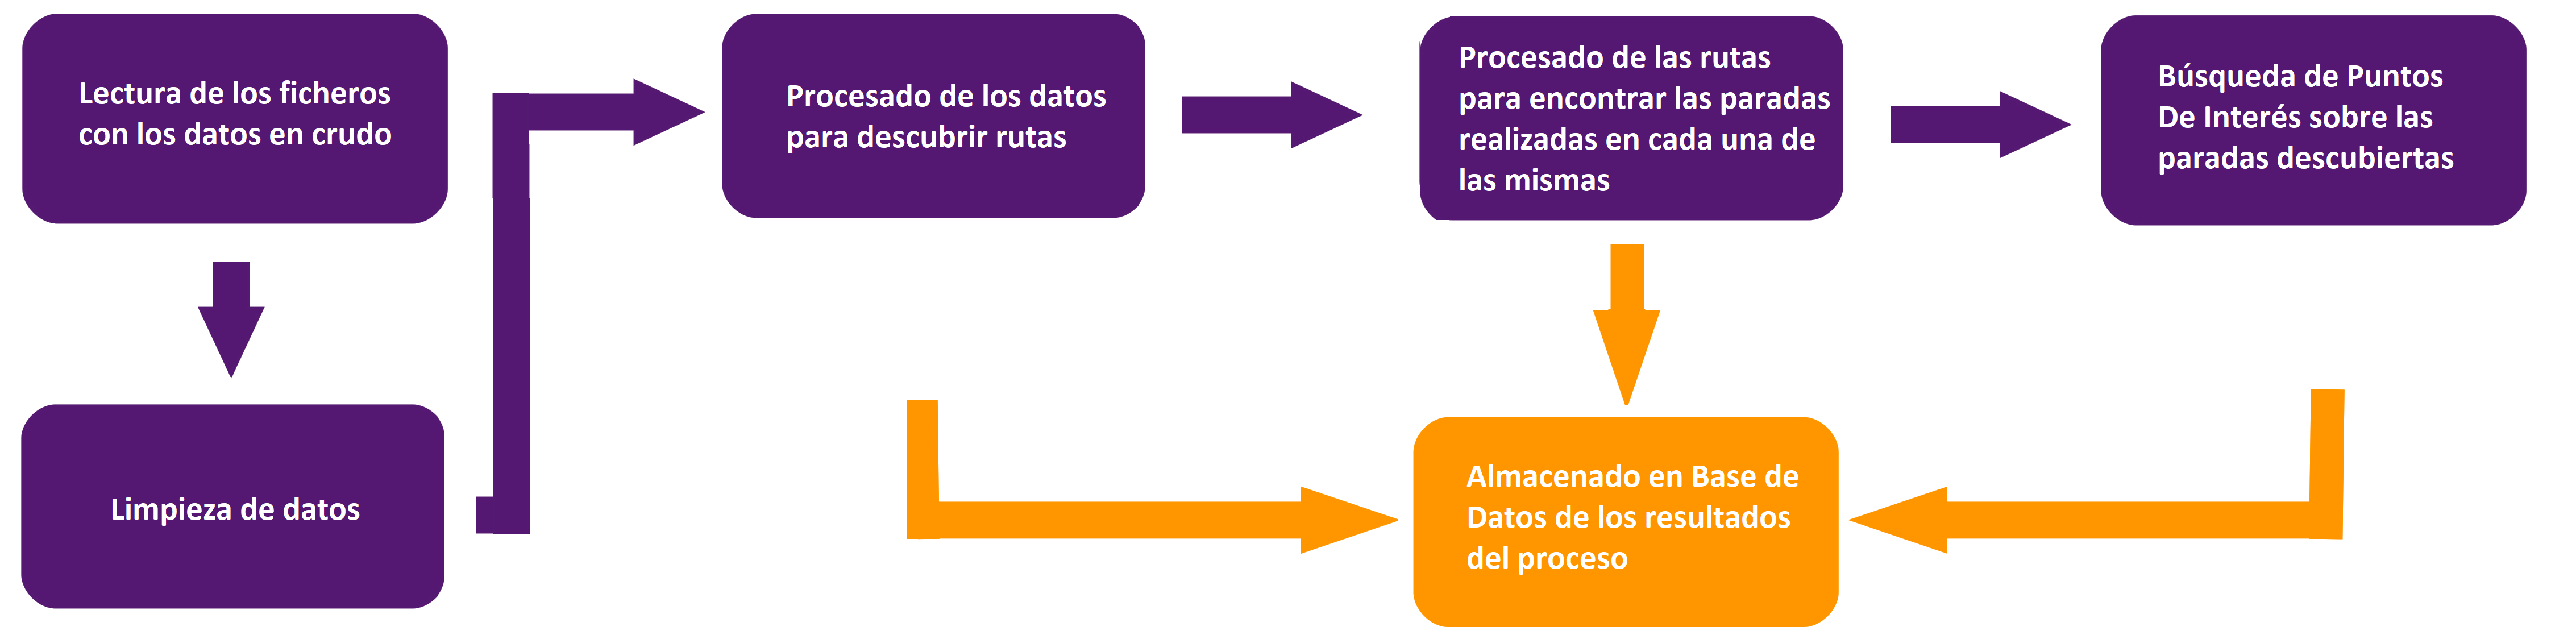
\includegraphics[width=1\textwidth]{../img/diagramas/algoritmo.png}
  \caption{Esquema del algoritmo.}
  \label{esquema}
\end{figure}

A continuación se explica cada uno de los puntos mencionados.

\subsection{Limpieza de datos}

Debido a fallos hardware o software, pueden capturarse rutas que no correspondan con la realidad. Este motivo implica la necesidad de un proceso previo de análisis de los datos para detectar posiciones que no son reales.

Algunos de los problemas que ocasionan que los datos deban pasar por una limpieza previa son los siguientes:

\begin{itemize}
	\item En ocasiones el hardware GPS puede fallar almacenando una posición errónea que no coincide con el resto de posiciones de la ruta.
	\item La precisión de los datos también puede verse afectada por una señal pobre en una zona con mala cobertura GPS.
	\item Este problema también puede ser ocasionado por el software al realizar mal alguno de los cálculos necesarios.
	\item Posiciones inexistentes por no cumplir con las características inherentes a una coordenada GPS. Por ejemplo, su longitud o latitud sobrepasen los límites (-90.0º - +90.0º para la latitud y -180.0º - +180.0º para la longitud).
	\item Falta de posiciones intermedias al haberse perdido la conexión y dándose una unión entre puntos de una ruta poco realista, generando una línea recta entre dos puntos cuando en condiciones normales dicha línea debería ser sustituida por puntos adicionales.
\end{itemize}

\subsubsection{Reconocimiento de rutas en cada fichero y asignación de área}
Una vez eliminadas las posibles posiciones irreales, el siguiente paso es el reconocimiento de las rutas que existen en el fichero analizado. Dentro de un fichero pueden convivir una o varias rutas dependiendo de la actividad del usuario. Estas rutas han de poder ser encontradas y reconocidas.

En este caso, el algoritmo trata de descubrir estas rutas mediante el cálculo de la mediana temporal aportado por cada marca de tiempo de las posiciones. Una vez obtenida dicha mediana, esta será comparada con las diferencias temporales entre todas las posiciones y, en el caso de encontrarse un gran salto temporal, se calculará el salto espacial entre las posiciones tan alejadas temporalmente. Si estas posiciones, además de estar separadas temporalmente, sobrepasan el umbral espacial marcado al algoritmo, las rutas se considerarán distintas y serán separadas.

Este cálculo se realizará con las rutas restantes y se obtendrá el total de rutas existentes en los ficheros analizados.

Una vez reconocida cada una de las rutas y, dependiendo de las opciones seleccionadas por el usuario, se asignará un área a dichas rutas.

Dependiendo de la opción, se seguirá uno de estos dos caminos:

\begin{itemize}
	\item Asignación de una área existente: se asignarán todas las rutas analizadas en la ejecución actual a un área ya existente en la Base de Datos. Esta opción es válida si se conoce cuál es el ámbito de las rutas analizadas y se tiene la certeza de que sus coordenadas cumplen con los límites del área seleccionada.
	\item Creación de una nueva área: el sistema creará un nuevo área con el nombre y descripción asignadas por el usuario. Las coordenadas se calcularán durante el análisis de las rutas.
\end{itemize}

\subsubsection{Segmentación de la trayectoria}

El siguiente paso consiste en dividir la trayectoria seguida en \quotes{movimiento} y \quotes{paradas}. Un periodo de movimiento es el tiempo en el que la persona se encuentra moviéndose entre dos ubicaciones mientras que un periodo de parada es el tiempo en el que, por ejemplo, la persona se encuentra viendo un lugar de interés.

Estas paradas son detectadas una vez calculada la mediana como se ha comentado en los puntos anteriores. En el caso de que existan posiciones cercanas espacialmente pero separadas en el tiempo, estas posiciones formarán una parada. Entendiendo como parada la entrada en un lugar de interés, la llegada y salida del puesto de trabajo de la persona que porta el dispositivo, etc.

De esta forma se obtienen paradas dentro de la ruta, contemplando el resto de posiciones como movimiento dentro de la misma.

\subsection{Enriquecimiento semántico}

El último proceso realizable es el correspondiente a la asignación de semántica a la ruta. Los datos obtenidos por el usuario solo incluyen posiciones geográficas tomadas en un instante determinado, es decir, solo se tienen datos como la latitud, longitud y el espacio temporal en el que han sido tomados. En esta etapa se incluye información adicional a estos datos.

Este proceso toma las paradas detectadas en la ruta y las contrasta con las posiciones de los Puntos De Interés almacenados en el sistema. Para ello se toma como límite el radio que marca la distancia máxima al que buscar un PDI.

Un PDI obtenido de Open Street Map puede contener diversa información, dicha información es aportada por la persona que registra dicho dato dentro de los sistemas OSM. Esta información incluye de forma obligatoria la posición espacial del Punto De Interés pero deja al usuario la posibilidad de añadir más información. Generalmente también se cuenta con un nombre en el idioma nativo de la persona que registra el PDI pero en otras ocasiones también existe un nombre genérico en inglés. Adicionalmente, un nodo suele incluir el tipo al que pertenece, este tipo recibe el nombre de \textit{amenity}. Una \textit{amenity} es una generalización de lugar al que representa el PDI. Por ejemplo, pueden existir museos, lugares de culto, gasolineras, centros comerciales, etc. De esta forma se puede conocer el nombre propio del lugar pero también qué tipo de lugar representa.

Una vez se han obtenido los PDIs cercanos a las paradas, todos los datos serán actualizados en la Base de Datos, permitiendo al usuario recuperarlos en el momento  que desee, mostrando los resultados en la página de resultados de la plataforma.

\capitulo{4}{Técnicas y herramientas}

Esta sección presenta un breve resumen de las técnicas y herramientas que han sido usadas para llevar a cabo este trabajo.

\section{Técnicas}

Las técnicas usadas en el desarrollo más relevantes son las mostradas a continuación.

\subsection{Modelo-Vista-Controlador}
Se ha hecho uso del patrón MVC para el desarrollo del proyecto. Este patrón permite la separación de la lógica de negocio de los datos y las vistas. Como su nombre indica, sus componentes quedan divididos en:

\begin{itemize}
	\item \textbf{Modelo:} representa los datos y la lógica de negocio.
	\item \textbf{Vista:} presenta la información del modelo.
	\item \textbf{Controlador:} controla las entradas del usuario y selecciona la vista.
\end{itemize}

\begin{figure}[h]
  \centering
    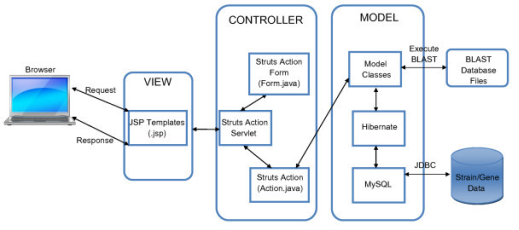
\includegraphics[width=0.6\textwidth]{../img/diagramas/mvc.png}
  \caption{Modelo-Vista-Controlador.}
  \label{ciclo}
\end{figure}

En el Anexo referente al Manual de Programación se detalla la estructura del proyecto según este patrón.

\subsection{Diseño Web Centrado en el Usuario}

A la hora de realizar una página web es fundamental tener en cuenta al usuario final de la misma, por tanto, siempre se ha de tener presente que la calidad de diseño es algo fundamental. El diseño de la plataforma modelará la interacción entre el usuario y la aplicación. De esta forma, un buen diseño, facilitará la consecución de los objetivos del usuario, mientras que un diseño pobre hará que el usuario busque otro medio por el que conseguir sus objetivos.

En esta sección se va a tratar el diseño centrado en el usuario, siguiendo el trabajo presentado en el trabajo realizado por Yusef Hassan-Montero, Francisco J. Martín Fernández y Ghzala Iazza \cite{montero:info}.

El citado trabajo explica y detalla en una serie de secciones todos los aspectos necesarios a la hora de diseñar, implementar y mantener un sitio web centrado en el usuario. Estas secciones son mostradas en la Figura \ref{ciclo} y descritas a continuación:

\begin{itemize}
	\item \textbf{Usabilidad y accesibilidad:} La ISO define usabilidad como: \quotes{Grado de eficacia, eficiencia y satisfacción con la que usuarios específicos pueden lograr objetivos específicos en contextos de uso específicos}. Aunque no siempre se va a poder dotar a la aplicación o plataforma de una usabilidad universal, es decir, que sea usable para todos los posibles tipos de usuarios, a la hora de diseñar dicha plataforma, se ha de tener en cuenta quiénes serán los usuarios potenciales y qué necesidades y conocimientos tienen.
	\item \textbf{Arquitectura de información:} La Arquitectura de la Información (AI) se puede definir como \quotes{el arte y la ciencia de organizar espacios de información con el fin de ayudar a los usuarios a satisfacer sus necesidades de información}. La actividad de organizar la información, incluye la estructuración, la clasificación y el rotulado de los contenidos de la aplicación.
	\item \textbf{Recuperación de la información:} El principal objetivo de un correcto diseño de la AI es que permita al usuario recuperar la información de la forma más sencilla posible.
	\item \textbf{Visibilidad:} El punto anterior está estrechamente ligado con la visibilidad de la información, es decir, que cada elemento de información pueda ser encontrado.
	\item \textbf{Diseño web centrado en el usuario:} 
El Diseño Web Centrado en el Usuario se caracteriza por asumir que todo el proceso de diseño y desarrollo de la plataforma ha de estar conducido por el usuario final y las necesidades y objetivos del mismo.
	\begin{itemize}
		\item \textbf{Planificación:} En este momento se han de identificar todos los objetivos, necesidades y requerimientos de la plataforma web. Se trata de encontrar un equilibrio entre las necesidades del usuario y lo que un programador puede ofrecer.
		\item \textbf{Diseño:} el diseño de una plataforma web se compone de:
		\begin{itemize}
			\item \textbf{Modelado del usuario:} se tratará de conocer las necesidades de los potenciales usuarios de
la aplicación.
			\item \textbf{Diseño conceptual:} tratará sobre el diseño de contenidos del portal web.
			\item \textbf{Definir el estilo:} se definirá el estilo de todo el sitio web.
			\item \textbf{Diseño visual:} trata de definir el número de colores que serán usados, el tipo de letra, etc.
			\item \textbf{Diseño de contenidos:} en este punto se valorará el contenido que cada sección mostrará al usuario.
		\end{itemize}
		\item \textbf{Prototipado:} cuenta cómo debe ser el prototipado de una aplicación web cualquiera, desde diseños básicos y sencillos hasta los prototipos idénticos a la versión final de la misma.
		\item \textbf{Evaluación:} indica las posibles formas de comprobar que el sitio web es \textit{usable}. 
		\item \textbf{Implementación:} trata sobre las cuestiones importantes a tener en cuenta durante la implementación de la plataforma como la escalabilidad y compatibilidad futura.
		\item \textbf{Mantenimiento y seguimiento:} refleja los aspectos más importantes a la hora de dar un mantenimiento a la plataforma web.
	\end{itemize}
	\item \textbf{Seguimiento de la usabilidad:} no todos los problemas de desarrollo habrán sido detectados antes de la puesta en producción del sistema, por tanto, es importante comprobar de forma constante que la plataforma funciona de forma correcta.
\end{itemize}


\begin{figure}[h]
  \centering
    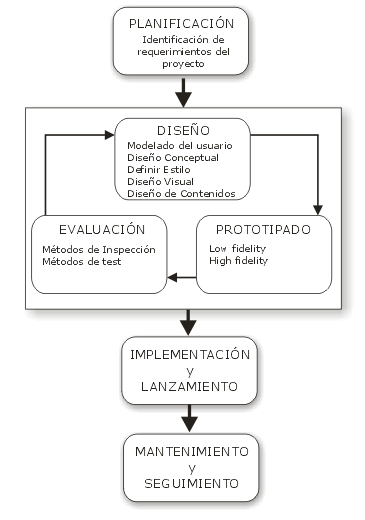
\includegraphics[width=0.6\textwidth]{../img/dwcu/ciclo.png}
  \caption{Esquema del diseño web centrado en el usuario.}
  \label{ciclo}
\end{figure}


\section{Herramientas}
Las herramientas usadas durante la implementación del proyecto se muestran en los siguientes apartados de esta sección.

\subsection{NetBeans}
El IDE elegido para el desarrollo del trabajo ha sido NetBeans \cite{netbeans:info} en su última versión disponible a la hora de finalizar este proyecto(8.2).

Este entorno ha sido elegido principalmente por haber sido usado en proyectos anteriores y poseer un conocimiento más avanzado del mismo que de otros entornos como puede ser Eclipse.

Atom ha sido usado como editor secundario para manejo de ficheros csv entre otros.

\subsection{Glassfish}
Para desplegar la aplicación web se cuenta con un servidor Glassfih en su versión 4.1 \cite{glass:info}.

\subsection{Open Street Map}
Open Street Maps (OSM) \cite{osm:wiki} es un proyecto colaborativo que permite crear y editar mapas. Estos mapas son de uso libre y gratuito para todos los usuarios, siendo solo los usuarios registrados los que pueden crear dichos mapas.

La creación de los mapas se lleva a cabo mediante la recogida de coordenadas geográficas usando dispositivos móviles. Estos dispositivos móviles obtendrán su ubicación gracias a sistemas GPS o Glonass o al uso de wifi o a la ubicación proporcionada por el operador de telefonía en caso de que el dispositivo cuente con una tarjeta SIM.

Los mapas son distribuidos bajo licencia ODbL (Licencia Abierta de Bases de Datos).

Los datos se almacenan siguiendo el datum WGS84 (World Geodetic System 1984, constituido por parejas latitud-longitud) usando la proyección de Mercator (definida en 1569  por Gerardus Mercator). La información primitiva consta de:

\begin{itemize}
	\item Nodos: son posiciones geográficas concretas.
	\item Vías: una lista ordenada de nodos constituye una vía. Esta puede ser una polilínea o un polígono.
	\item Relaciones: son grupos de vías, nodos y relaciones que pueden ser agrupadas ya que contienen propiedades comunes.
	\item Etiquetas: son usadas para almacenar metadatos sobre los objetos del mapa, constan de una pareja clave-valor. 
\end{itemize}

\subsection{PostgreSQL 9.6}
PostgreSQL \cite{post:info} es un Sistema Gestor de Bases de Datos (SGBD) relacional, orientado a objetos y libre, distribuído bajo licencia PostgreSQL License. Actualmente se encuentra en su versión 9.6 siendo la usada en este trabajo.

\subsection{PostGIS}
PostGIS \cite{postgis:wiki} es una Base de Datos espacial que expande las posibilidades de PostgreSQL añadiendo soporte a objetos geográficos permitiendo consultas de localización. PostGIS ha sido diseñado y desarrollado por la empresa Refraction Research siendo distribuido bajo licencia GNU (GPLv2).

\subsection{QGIS}
Para los pasos previos de este trabajo se ha hecho uso del programa QGIS \cite{qgis:info}. QGIS es un sistema de información geográfico libre y de código abeirto. Cuenta con una infinidad de opciones, algunas de las más relevantes son:

\begin{itemize}
	\item Conexión con PostgreSQL: permite mantener una conexión contra la Base de Datos que contiene los datos relativos a los análisis de las rutas. De esta forma es posible pintar sobre un mapa todos y cada uno de los puntos de cada ruta analizada. Es posible adaptar las consultas SQL para obtener la información deseada antes de ser pintada.
	\item Uso de diferentes APIs de mapas: permite usar mapas de Open Street Maps, Google Maps, etc.
	\item Descarga de datos OSM: permite la descarga de datos en formato osm indicando el área deseado.
\end{itemize}

\subsection{Osmosis}
Osmosis \cite{osmosis:info} es una herramienta desarrollada en Java y que funciona por línea de comandos. Permite procesar ficheros OSM con un gran rendimiento debido a que está diseñada para tratar con ficheros de extensión considerable (un fichero osm conteniendo información completa de un país puede superar los 10 GiB de datos).

Esta herramienta permite desde cargar datos sobre una Base de Datos hasta extraer un subconjunto de ellos a partir de un fichero de tipo osm. Además, Osmosis puede formar parte de otras aplicaciones Java incluyéndose como una librería.

\subsection{Osmconvert} \cite{osmconvert:wiki}
Esta herramienta permite realizar distintas conversiones entre ficheros de distinta extensión. En el caso de este proyecto, la herramienta permite al usuario transformar ficheros de extensión pbf a ficheros osm con los que trabajar posteriormente.

\subsection{Osmfilter} \cite{osmfilter:wiki}
Como su nombre indica, la herramienta Osmfilter permite filtrar ficheros osm mediante sus etiquetas. En este trabajo ha sido usada para extraer ficheros de tipo XML a partir de ficheros de extensión osm manteniendo únicamente los Puntos De Interés del área englobada en el fichero original.

\subsection{\LaTeX}
Se ha usado \LaTeX  para la realización de la documentación del presente Trabajo de Fin de Máster. El contenido ha sido editado con TexMaker en su versión 4.5.

\subsection{Lenguajes de programación, marcado y/o SQL}

\subsubsection{HTML 5}
HyperText Markup Lenguage 5 es la última versión del estándar HTML publicado a finales del año 2014 siendo sucesor de la versión 4.01. Incluye nuevas etiquetas dejando otras obsoletas. Es un lenguaje de marcado destinado al desarrollo de páginas web. Es un lenguaje estándar que cualquier navegador web será capaz de reconocer e interpretar.

\subsubsection{Java}
Java es un lenguaje de programación orientado a objeto concurrente y de propósito general. Java mantiene un número de dependencias reducido para permitir la ejecución del programa desarrollado en el mayor número de dispositivos posibles sin ser recompilado.

La primera revisión de este lenguaje fue desarrollada por James Gosling en la ya desaparecida Sun Microsystems (actualmente absorbida por Oracle), siendo cada aplicación Java compilada y ejecutada por una máquina virtual Java (JVM).

Aunque este lenguaje apareció en 1995, no fue hasta 2012 cuando se convirtió en uno de los lenguajes más usados, especialmente en aplicaciones cliente-servidor. La versión estable actual es la 8.

\subsubsection{Servlet}

Un servlet \cite{servlet:wiki} es un componente ubicado en el servidor Java EE encargado de dar respuesta a las peticiones de los clientes. Cada servlet amplía las capacidades del servidor en el que se encuentra pudiendo generar contenido dinámico como pueden hacer PHP o ASP.NET.

El ciclo de vida de un servlet es el siguiente:

\begin{itemize}
	\item Inicialización: el proceso de inicialización (llamada al método init) ha de hacerse antes de que el servlet pueda interaccionar con los clientes.
	\item Interacción: una vez inicializado, el servlet, puede atender a las peticiones de los clientes.
	\item Destrucción: para destruir un servlet se ha de llamar a su método destroy. Este método será llamado cuando el servidor sea cerrado o el administrador del sistema lo requiera. Para inicializar el servlet destruido se ha de llamar al método init de nuevo.
\end{itemize}

\subsubsection{JSP}
Java Server Pages o JSP \cite{jsp:wiki} es una tecnología de vistas que corre en el lado del servidor permitiendo escribir plantillas en lenguajes como HTML, JavaScript o CSS. Una página JSP puede contener segmentos de código implementados en Java que permitan modelar dicha página de forma dinámica.

Una de las ventajas de JSP es su base en Java, permitiendo crear clases de acceso a datos (DAO), lógica de negocio, etc.

Una página JSP permite sintaxis como la siguiente:

\begin{itemize}
	\item Directivas: permiten incluir otros ficheros, clases Java para el manejo de objetos, etc.
	\item Declaraciones: permiten declarar variables, funciones y datos estáticos.
	\item Expresiones: permiten evaluar expresiones Java.
	\item Etiquetas: simplifican el código aportando funcionalidad añadida. Existen dos grandes grupos de etiquetas: las que proporcionan funcionalidad a la página (como jsp:include) y las que permiten manipular componentes JavaBean (como jsp:useBean).
	
\end{itemize}

\subsubsection{CSS 3}
Cascading Style Sheet (CSS) es un lenguaje usado para definir la presentación visual de un documento escrito en HTML y  permitiendo separar la estructura de un documento de su presentación. El estilo puede ser incorporado \quotes{en línea}, mediante una hoja interna o mediante el uso de una hoja de estilo externa.

El principal problema que persiste con el paso de las versiones es el centrado vertical ya que no es sencillo y requiere de más reglas que el centrado horizontal (siendo este último casi automático).

\subsubsection{Bootstrap 3}

Esta plataforma web se ha diseñado pensando en el usuario final de la misma, por tanto, se han tenido en cuenta las pautas marcadas por un diseño adaptable (Responsive Web Design). Este objetivo ha sido posible gracias al uso de un framework como Bootstrap. Este framework permite diseñar el sitio para todos los tamaños de pantalla actuales.

Bootstrap \cite{boot:info} implementa CSS para una gran cantidad de clases, lo que hará que el diseño de la plataforma web sea más sencillo. Unas de las clases más importantes son las que permiten adaptar el contenido mostrado al tamaño de pantalla desde la que la web ha sido accedida.

En Bootstrap el contenido se agrupa en filas (row) y en columnas (col) hasta un máximo de 12 columnas. Por tanto, en las líneas superiores, se crea una fila (row) y el div interno especifica las columnas para un tamaño de pantalla xs o md (estos tamaños ya están predefinidos en Bootstrap). De esta forma tan sencilla se puede agrupar el contenido de ese \quotes{div} mediante el CSS que ya contiene el framework. 

Bootstrap también contiene gran cantidad de estilos para menús, botones, listas, además de colores recibiendo el nombre de componentes. Se pueden encontrar iconos que se podrán usar en botones, en texto, menús de usuario simples o con accesos desplegables, mensajes de alerta con colores llamativos para el usuario, barras de progreso, etc.

\subsubsection{JavaScript y jQuery}

JavaScript (JS) es un lenguaje interpretado, débilmente tipado y dinámico, que cumple el estándar ECMAScript siendo la última versión estable la ECMAScript 2016. En el desarrollo de una página web, se usará en el lado del cliente, permitiendo la generación de páginas dinámicas o la mejora de la interfaz de usuario. En la actualidad, la gran mayoría de los navegadores son capaces de interpretar este lenguaje. JavaScript está provisto de una implementación del DOM (Document Object Model) para poder interactuar con la página web.

Aunque se pueda pensar que Java y JavaScript están relacionados, en realidad, no es así. Inicialmente JavaScript fue diseñado con una sintaxis similar a C aunque adoptando nombres y convenciones similares a las de Java.

jQuery es una biblioteca de JavaScript (presentada en enero de 2006) que pretende simplificar la interacción con los documentos HTML, la manipulación del DOM o el manejo de eventos. Además de permitir una interacción con la técnica AJAX.
En la misma web que la usada para JavaScript se pueden encontrar gran variedad de ejemplos y referencias para el uso de jQuery

En jQuery, se usa la función \$ para interaccionar con las páginas HTML. Recibe como parámetro el nombre de una etiqueta HTML o una expresión en CSS, devolviendo todos los nodos del DOM que concuerdan con esa expresión. Si queremos que esto funcione en Drupal, tenemos que dar un paso más, y es que debemos englobar esta función dentro de otra.

\subsubsection{AJAX}
Asynchronous JavaScript And XML, conocida como AJAX, es una técnica de desarrollo web que permite la implementación de aplicaciones interactivas. Las aplicaciones se ejecutarán en el navegador del cliente y, por detrás, se mantiene una comunicación asíncrona con el servidor. Así, es posible, que la página sea actualizada sin necesidad de realizar una recarga completa de la misma. Con AJAX, se mejora la interactividad, velocidad y usabilidad de estas aplicaciones. AJAX no es una tecnología en sí sino un término que engloba a un conjunto de las mismas que trabajan de forma conjunta. HTML y CSS: para la presentación de la información. Document Object Model (DOM): para mostrar la información e interaccionar con la misma. JSON: para intercambiar datos. XMLHttpRequest: para poder mantener una comunicación asíncrona. JavaScript: para unir estas tecnologías. En la siguiente página web podemos encontrar mucha información relativa tanto a JavaScript como a AJAX en particular.

\subsection{Máquina virtual y sistema operativo}
Se ha optado por instalar el Sistema Operativo Ubuntu 16.04 LTS en una máquina virtual bajo el entorno de Virtual Box. De esta forma, se permite exportar e importar la máquina pudiendo ser instalada en cualquier ordenador. Además, este planteamiento permite hacer uso de la plataforma web de forma offline y sin tener que estar disponible en un servidor.

Además se ha hecho uso de diversos navegadores web como son Chrome, Firefox o Konqueror, para poder comprobar el correcto funcionamiento del sitio, además de la correcta visualización del contenido de la hoja de estilo. Es un punto importante ya que algunos navegadores, en versiones antiguas, puede que no soporten todas las etiquetas del estándar HTML5 o todo los correspondientes estilos de CSS3.

\capitulo{5}{Aspectos relevantes del desarrollo del proyecto}

A la hora de realizar un proyecto de este tipo siempre surgen problemas o cuestiones que se han de ir resolviendo en ese momento, esta sección trata los puntos más relevantes.

\section{Concepto inicial del proyecto}
El proyecto planteado, en su forma inicial, trataba de la implementación de una aplicación de escritorio en lenguaje Python o Java permitiendo asignar semántica a las rutas analizadas.

Para ello, la aplicación debería poder leer y procesar ficheros de texto plano o csv. Todos los datos obtenidos serían almacenados en una Base de Datos PostgreSQL puesto que cuenta con una extensión llamada PostGIS que permite el análisis y tratamiento de posiciones geográficas añadiendo funcionalidad adicional al SGBD mencionado.

Puesto que la aplicación debía ser de fácil uso, se planteó una interfaz basada en Swing para poder mostrar los datos analizados así como mapas con las rutas procesadas.

Los primeros pasos orientados al diseño de la interfaz mediante Swing dejaron claro que no era la más adecuada ni sencilla para trabajar con mapas. Este es uno de los aspectos que animó a abandonar esta idea inicial por un desarrollo web cuya interfaz permite un manejo mucho más sencillo de todo tipo de mapas y librerías.

\section{Conocimientos previos}
A la hora de realizar este trabajo se contaban con algunos conocimientos previos  de programación web obtenidos a lo largo de los distintos cursos universitarios así como del desarrollo del Trabajo de Fin de Grado (basado en el CMS Drupal).

Aunque en esta ocasión el lenguaje elegido fue Java y se completó el desarrollo haciendo uso de páginas JSP y servlets. Por tanto, se tuvo que realizar un esfuerzo para aprender el manejo y programación mediante este lenguaje.

Adicionalmente, no se contaban con conocimientos sobre el funcionamiento de los sistemas de obtención de coordenadas ni de cómo podían ser tratados posteriormente.


\subsection{Coordenadas geográficas}
Debido a los distintos tipos de toma y representación de coordenadas geográficas es posible que una misma coordenada representada sobre distintos sistemas de mapas de lugar a errores de representación de varios centenares de metros. Este comportamiento puede observarse al comparar coordenadas geográficas presentadas por distintos motores de mapas. Por ejemplo, una coordenada localizada en China mostraba un mapa basado en Open Street Map no coincidirá con la misma coordenada mostrada por los mapas de Google.

Esto es así por el uso de distintos sistemas de coordenadas usados por ambos motores (EPSG:3857 en Google Maps frente a EPSG:4326 en OpenStreetMaps) \cite{epsg:wiki}.

Al comienzo del desarrollo del trabajo, no se conocían los diferentes sistemas de coordenadas dando lugar a confusión y errores en los cálculos sobre las rutas.

La Figura \ref{coordenadas} muestra la gran cantidad de sistemas de coordenadas disponibles a la hora de visualizar un fichero de puntos GPS o a la hora de obtener datos desde PostgreSQL.


\begin{figure}[h]
  \centering
    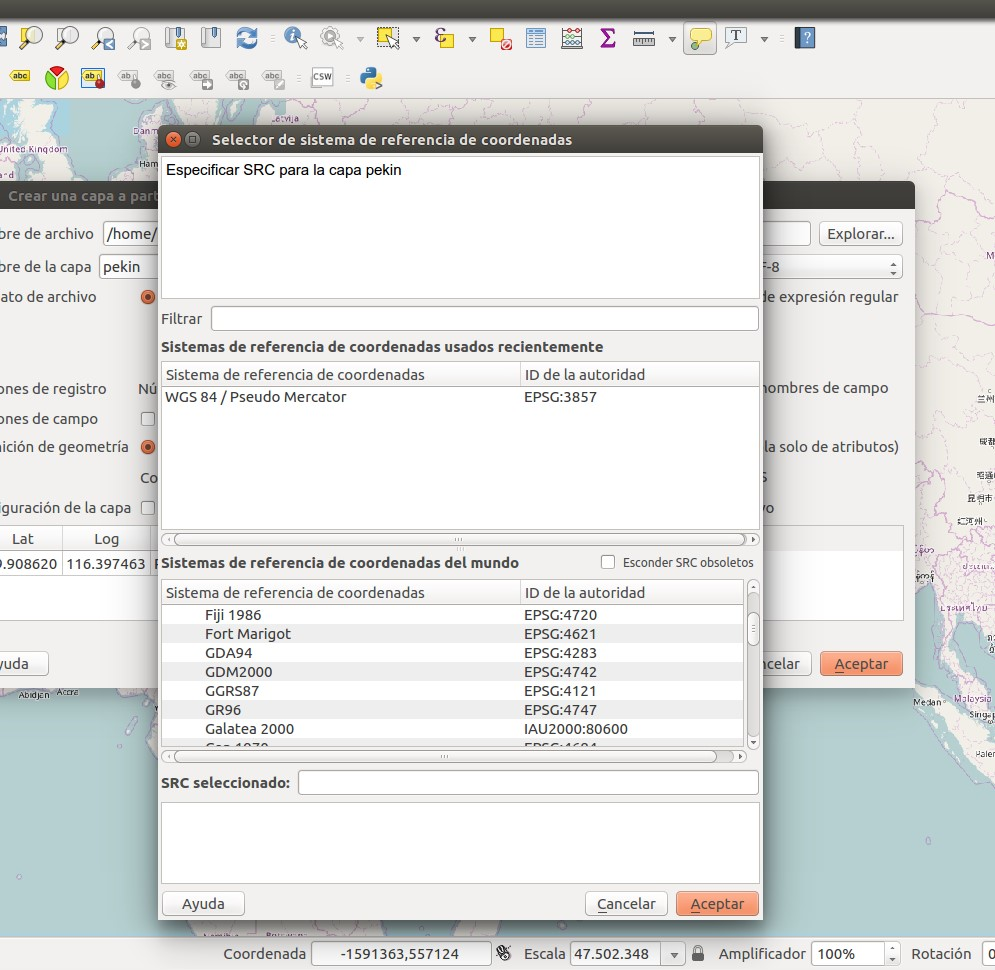
\includegraphics[width=0.6\textwidth]{../img/poi/qgis.jpg}
  \caption{Gran cantidad de sistemas de coordenadas en QGIS.}
  \label{coordenadas}
\end{figure}

\section{Errores propios del hardware}
Toda la tecnología GPS relacionada con el hardware cuenta con ciertas limitaciones, tanto en potencia de cálculo como en la toma de las posiciones en sí mismas.

Estas limitaciones favorecen la aparición de errores en las coordenadas medidas por cualquier hardware. Estos errores pueden hacer que la ruta tomada como verdadera contenga pequeños fallos en cada una de las coordenadas de las que está compuesta. Por este motivo, puede que una ruta inicialmente correcta indique un espacio recorrido mayor al realmente realizado o, incluso, marque puntos por los que no se han pasado.

Este echo puede ser fácilmente verificado atendiendo a las restricciones inherentes del hardware y a la forma en la que el software es implementado. Dejando un dispositivo GPS activo en un punto fijo, se verá al cabo de un cierto espacio de tiempo que el dispositivo parece moverse de forma autónoma. Este movimiento viene dado por los errores y/o fallos mencionados anteriormente.

Por tanto, es posible afirmar, que los datos con los que cada usuario cuenta tendrán un cierto error. Esto hace que los algoritmos de análisis y muestra de resultados deban tolerar estas inexactitudes. La Figura \ref{errores} muestra el movimiento virtual efectuado por dispositivo GPS completamente parado. \cite{pais:info}

\begin{figure}[h]
  \centering
    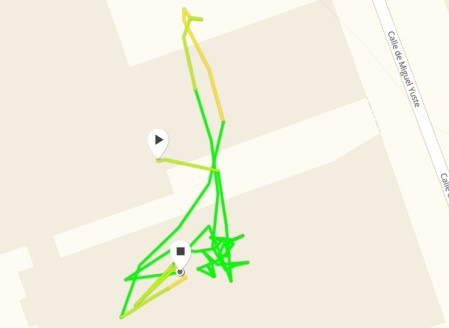
\includegraphics[width=0.6\textwidth]{../img/gps/errores.jpg}
  \caption{Movimiento }
  \label{errores}
\end{figure}

Estas restricciones han ocasionado que algunos conjuntos de datos no cuenten con la calidad suficiente para su uso en este trabajo así como que sus errores sean tan cuantiosos que las rutas no sean verosímiles.

\section{Obtención de datos}
Uno de las primeras cuestiones a resolver fue la búsqueda de datos que permitiesen dar comienzo al desarrollo del proyecto. Aunque existen gran variedad de \textit{datasets} en diversas páginas web dedicadas a su alojamiento, es cierto que no siempre cumplían con los requisitos necesarios para proceder a su análisis.

Algunos conjuntos de datos contaban con un buen número de ellos pero no contaban con ciertas características como una marca temporal para cada coordenada geográfica. Otros contaban con un buen número de características pero, en conjunto, resultaba un tamaño demasiado pequeño como para ser analizado.

Finalmente se encontró un conjunto de datos de Microsoft que, de forma general, satisfacía los requisitos que se habían marcado como mínimos siendo el usado para llevar a cabo las pruebas del sistema.

En este momento también comenzaron a surgir algunos de los problemas como los  que se indican en apartados inferiores.


\section{Tamaño de los datos de análisis}
Como ya ha sido comentado con anterioridad, el proyecto ha sido basado en una máquina virtual. Inicialmente se otorgó un tamaño estándar y fijo para el correcto desempeño de la distribución elegida. Pronto se tuvo constancia de que este tamaño no era suficiente. Aunque ya se habían instalado y configurado todos los componentes necesarios para el proyecto (PostgreSQL, PostGIS, NetBeans, etc.) no hubo otra opción que volver a crear una nueva máquina, esta vez con un tamaño mucho mayor y de espacio dinámico. Una vez reconfigurado todo el software necesario se pudo continuar con el normal desarrollo del trabajo.

No obstante y, como se describe a continuación, no solo crecía el tamaño en disco de todo el sistema, sino que también la Base de Datos aumentaba su volumen.

Antes de comenzar con las pruebas del sistema se cargó la Base de Datos con un completo conjunto de datos del mapa de China (los datos usados para las pruebas estaban basados en su gran mayoría en la ciudad de Pekín) viendo que el tamaño de las tablas era tan grande que ralentizaba cualquier intento de análisis de rutas.

En este momento se estaba llegando al límite de recursos de hardware que se podían asignar a la máquina virtual (llegando a contar con hasta 8 hilos, 10 GiB de RAM y un tamaño superior a las 100 GiB de espacio en disco). Se debía considerar otra aproximación que lograse una mejor experiencia y un mejor rendimiento.

Pronto se tuvo claro que no era necesaria tan elevada cantidad de datos y, que realmente, solo se usarían datos pertenecientes a la capa de Puntos De Interés. Es en este punto en el que se buscan herramientas para extraer estos PDIs de los ficheros de tipo osm descargados inicialmente. En esta búsqueda se encuentran las herramientas mencionadas en la sección anterior (Técnicas y herramientas).

De esta forma se logra disminuir el tamaño de unas tablas excesivamente grandes logrando una mejora del rendimiento global del sistema. Una vez iniciadas las pruebas del análisis de rutas del sistema se comprueba que el rendimiento ha experimentado una mejora real y se decide optar por mantener la estructura y conjunto de datos usados hasta el momento.


Como cabe esperar si finalmente la plataforma es puesta en producción, se hará uso de un servidor apropiado y con capacidades suficientes para que todo el sistema se comporte de forma correcta quedando disipado este problema .


\section{Tiempos de ejecución}
Ligado a los problemas mostrados en los apartados anteriores, los tiempos de ejecución eran tan elevados que, inicialmente, se necesitaban varias horas para obtener los primeros resultados. En estos momentos el hardware había llegado a su límite y no era posible una mayor asignación de recursos.

Una vez reducido el tamaño de los datos a consultar el rendimiento aumentó de forma considerable y ahora se pueden obtener los resultados esperados en pocos minutos.


\section{Diseño del algoritmo}
Durante los primeros pasos del proyecto se diseñó un algoritmo que incluía todos los pasos del mismo de forma secuencial. Es decir, todos los pasos debían ser ejecutados una vez se lanzase.

Este comportamiento no es el ideal puesto que el usuario puede tener la oportunidad de elegir los pasos que desea realizar sobre los datos que contienen sus ficheros. Por ejemplo, puede desear que sus datos no se mantengan en el sistema, que una ejecución busque PDIs pero otra solo paradas, etc.

Por tanto se decidió separar el algoritmo en diferentes clases que permitiesen una ejecución del algoritmo más personalizada.

Este hecho hizo que el desarrollo se viese ralentizado puesto que el cambio de la implementación del algoritmo implicó más tiempo del planeado inicialmente. Además, en este momento, se llevó a cabo la migración hacia la plataforma web, lo que implicó cambios adicionales sobre el código.


\capitulo{6}{Estado del arte}

En este apartado se va a aportar una visión más amplia del \quotes{estado del arte} mediante el estudio de otras herramientas similares.

\section{Weka-STPM}
WEKA for Moving Object Data Analysis and Mining o Weka-STPM es una extensión para Weka que permite soportar de forma automática el procesado de trayectorias o rutas para añadir semántica a las mismas. Está desarrollada por la Doctora Vania Bogorny, profesora del Departamento de Informática y Estadística en la Universidad Federal de Santa Catarina (Brasil).

Inicialmente parece una herramienta clave que podía haber facilitado el análisis de las rutas puesto que permitía la lectura y escritura en Bases de Datos PostgreSQL y soportaba la extensión PostGIS, pero tras algunas pruebas se vio que no se obtenían los resultados esperados.

Además, se puede ver por su código, que no está completamente terminada, encontrándose algunos errores en su ejecución y opciones no disponibles. Por ejemplo, aunque se lograba una conexión contra la Base de Datos, no se lograba que la aplicación insertase ningún tipo de resultado en la misma.

Su interfaz (Figura \ref{weka}) basada en Swing tampoco ayuda a comprender su funcionamiento puesto que hay botonoes que quedan ocultos, opciones que no se visualizan y desplegables que desaparecen detrás del resto de menús. Ante los problemas encontrados no se puede afirmar que esta herramienta pueda ser de gran utilidad en la actualidad pero sí es posible garantizar que si su desarrollo finaliza supondrá un gran paso adelante en el análisis de cualquier tipo de trayectoria.

\begin{figure}[h]
  \centering
    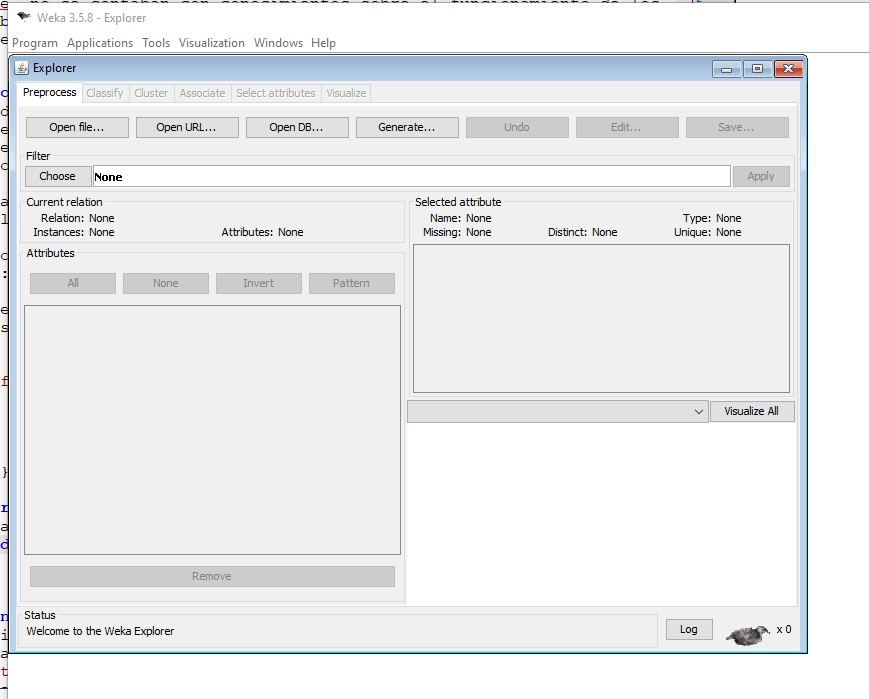
\includegraphics[width=0.6\textwidth]{../img/weka/weka.jpg}
  \caption{Interfaz sencilla de weka.}
  \label{weka}
\end{figure}


\section{CARTO}
Carto es una plataforma de cómputo en la nube SaaS (Software as a Service) que provee de un sistema de información geográfica o GIS y herramientas de mapeo de información para navegadores web.

Está basada en la extensión PostGIS de ProstreSQL y es de código abierto. Su \textit{front-end} está basado en JavaScript mientas que su \textit{back-end} está basado en Node.js.

El aspecto que muestran los mapas creados mediante CARTO puede ser visto en la Figura \ref{carto}.

\begin{figure}[h]
  \centering
    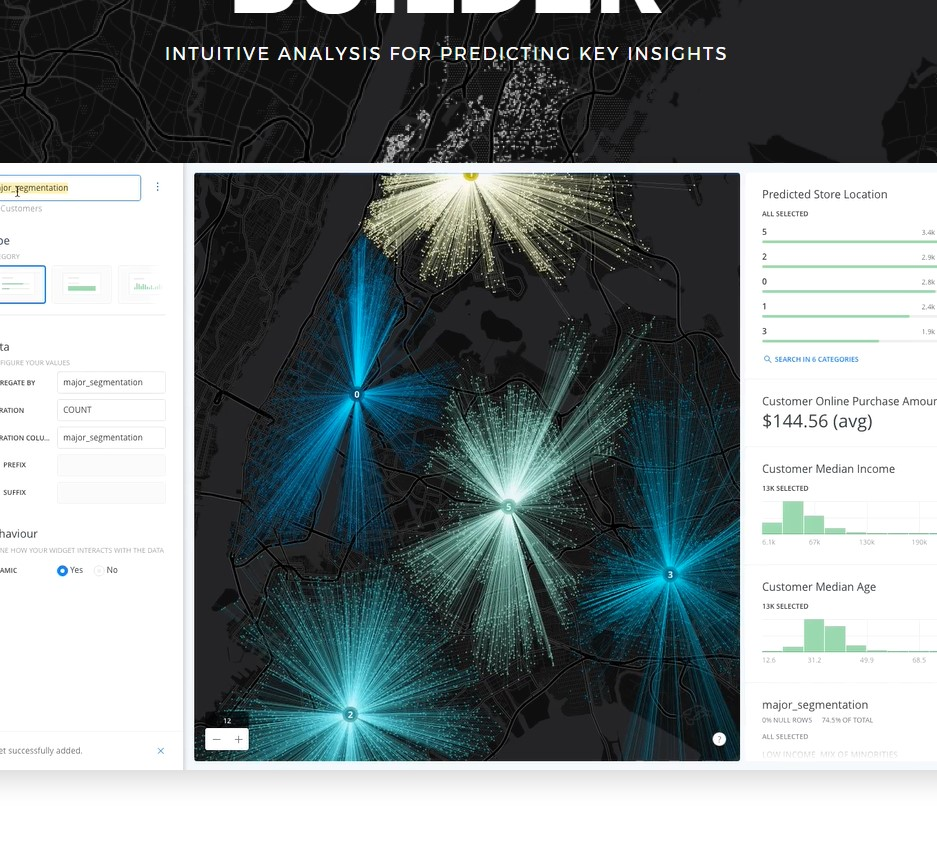
\includegraphics[width=0.6\textwidth]{../img/weka/carto.jpg}
  \caption{Aspecto final de los mapas en CARTO.}
  \label{carto}
\end{figure}


\subsection{CARTO Builder}
CARTO Builder es una aplicación web en la que los usuarios pueden procesar sus datos, realizar anaálisis y diseñar mapas propios. CARTO Builder está pensado y diseñado para todas las personas noveles que desean hacer uso de estas herramientas sin contar con conocimientos previos ni avanzados en sistemas de información geográficos. No obstante se provee de acceso a consultas SQL que pueden ser personalizadas si se cuenta con mayores conocimientos.

\subsection{CARTO Engine}
CARTO Engine provee al usuario de distintas APIs y librerías que permiten la construcción de mapas completamente personalizados.

\begin{itemize}
	\item SQL: se pueden hacer uso de todas las sentencias SQL soportadas en PostgreSQL.
	\item Mapas: permite obtener distintas plantillas de mapas en base a los requerimientos del usuario. De esta forma, cada usuario puede diseñar un mapa propio que usar en una aplicación web.
	\item Servicio de datos: permite desarrollar una mayor funcionalidad como el \textbf{geocoding}.
\end{itemize}

Aunque como se puede apreciar, su gran variedad de características permite una amplia capacidad de análisis de datos pudiendo ser una herramienta potente y de interesante uso, no se adapta al completo a los requerimientos iniciales de este proyecto, por lo que se decidió no hacer uso de la misma.

\section{Google Trips}

Quizá la primera aproximación a esta aplicación pueda parecer que es la que más se adapta al espíritu de este proyecto. Google Trips (Figura \ref{trips}) permite organizar viajes o rutas en pocos minutos.

También facilita obtener sugerencias de sitios no visitados que guardan relación con los visitados anteriormente y que hayan gustado a su usuario, preparar rutas diarias, organizar reservas según un calendario en Gmail, etc.

\begin{figure}[h]
  \centering
    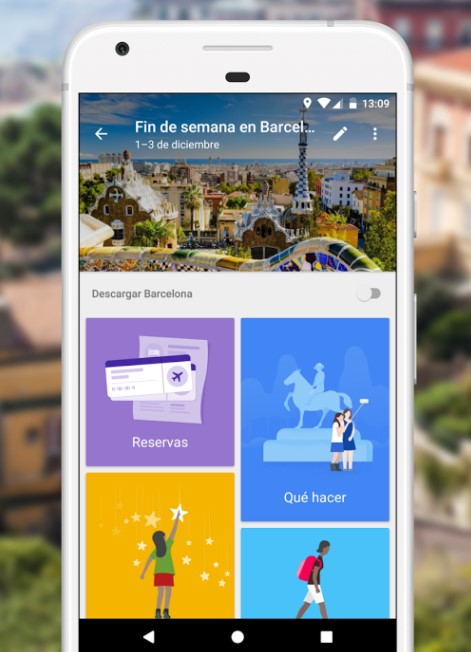
\includegraphics[width=0.6\textwidth]{../img/weka/trips.jpg}
  \caption{Aspecto de la interfaz de la aplicación Google Trips.}
  \label{trips}
\end{figure}

Pero el aspecto que esta aplicación móvil no realiza es el análisis y asignación de semántica a rutas ya realizadas, aspecto que diferencia la plataforma desarrollada con esta aplicación.


\section{Conclusiones sobre el estado del arte}

Como se ha visto en los apartados anteriores, existe una variedad interesante de plataformas y/o aplicaciones desarrolladas con el afán del análisis y/o gestión de rutas basadas en coordenadas GPS. Si bien existen más plataformas similares a las mencionadas, en esta sección se han mostrado las juzgadas como más interesantes.

Comparando sus características se puede ver que estas plataformas no permiten asignar semántica a trayectorias basadas en coordenadas geográficas. Por tanto, se puede afirmar que por los ejemplos mostrados en esta sección de la documentación, la aplicación web aquí mostrada añade nuevas funcionalidades a los sistemas existentes.

Por último, cabe destacar que, la plataforma desarrollada está completamente basada en tecnologías y datos libres de los que cualquier usuario puede hacer uso.



\capitulo{7}{Conclusiones y Líneas de trabajo futuras}

Todo proyecto debe incluir las conclusiones que se derivan de su desarrollo. Éstas pueden ser de diferente índole, dependiendo de la tipología del proyecto, pero normalmente van a estar presentes un conjunto de conclusiones relacionadas con los resultados del proyecto y un conjunto de conclusiones técnicas. 
Además, resulta muy útil realizar un informe crítico indicando cómo se puede mejorar el proyecto, o cómo se puede continuar trabajando en la línea del proyecto realizado. 


\section{Conclusiones}

\section{Lineas de trabajo futuras}



\bibliographystyle{plainnat}
\bibliography{bibliografia}

\end{document}